\documentclass[11pt,a4paper]{article}

% Essential packages for math
\usepackage{amsmath,amssymb,amsthm}
\usepackage{mathtools}
\usepackage{bm}

% Page layout
\usepackage{geometry}
\geometry{margin=1in}

% Graphics and colors
\usepackage{graphicx}
\usepackage{xcolor}
\usepackage{tikz}
\usepackage{pgfplots}
\pgfplotsset{compat=1.17}
\usetikzlibrary{shapes.geometric, arrows.meta, calc, patterns, positioning, decorations.pathmorphing}

% Tables
\usepackage{booktabs}
\usepackage{multirow}
\usepackage{array}
\usepackage{longtable}

% Algorithms
\usepackage{algorithm}
\usepackage{algorithmicx}
\usepackage{algpseudocode}

% Code listings
\usepackage{listings}
\lstset{
    basicstyle=\ttfamily\small,
    breaklines=true,
    frame=single,
    numbers=left,
    numberstyle=\tiny,
    keywordstyle=\color{blue},
    commentstyle=\color{green!50!black},
    stringstyle=\color{red},
    showstringspaces=false
}

% References and links
\usepackage{hyperref}
\hypersetup{
    colorlinks=true,
    linkcolor=blue,
    citecolor=green,
    urlcolor=red
}

% Other useful packages
\usepackage{enumerate}
\usepackage{enumitem}
\usepackage{subcaption}
\usepackage{float}
\usepackage{wrapfig}

% Theorem environments
\theoremstyle{definition}
\newtheorem{definition}{Definition}[section]
\newtheorem{theorem}{Theorem}[section]
\newtheorem{lemma}[theorem]{Lemma}
\newtheorem{proposition}[theorem]{Proposition}
\newtheorem{corollary}[theorem]{Corollary}
\newtheorem{remark}{Remark}[section]

% Custom commands
\newcommand{\E}{\mathbb{E}}
\newcommand{\R}{\mathbb{R}}
\newcommand{\N}{\mathcal{N}}
\newcommand{\KL}{\text{KL}}
\newcommand{\ELBO}{\text{ELBO}}
\DeclareMathOperator{\Var}{Var}

\title{\Large \textbf{Denoising Diffusion Probabilistic Models (DDPM):\\A Comprehensive Mathematical Treatment}}
\author{LaTeX Functionality Test Document\\Inspired by "What are Diffusion Models?" by Lilian Weng}
\date{\today}

\begin{document}

\maketitle

\begin{abstract}
This document provides a comprehensive mathematical treatment of Denoising Diffusion Probabilistic Models (DDPMs), demonstrating various LaTeX functionalities including complex mathematics, algorithms, visualizations, tables, and code listings. We explore the theoretical foundations, derive key equations, and implement core algorithms while showcasing LaTeX's typesetting capabilities.
\end{abstract}

\tableofcontents
\newpage

\section{Introduction}

Diffusion models are a class of generative models that learn to gradually denoise data by reversing a diffusion process. Given data distribution $q(\mathbf{x}_0)$, we define a \textit{forward diffusion process} that gradually adds Gaussian noise over $T$ timesteps:

\begin{equation}
    q(\mathbf{x}_t | \mathbf{x}_{t-1}) = \N(\mathbf{x}_t; \sqrt{1-\beta_t}\mathbf{x}_{t-1}, \beta_t\mathbf{I})
    \label{eq:forward_step}
\end{equation}

where $\{\beta_t\}_{t=1}^T$ is a variance schedule with $\beta_t \in (0,1)$.

\subsection{Key Contributions}

The main contributions of DDPM can be summarized as:

\begin{itemize}[leftmargin=*]
    \item \textbf{Simplified training objective}: Connection to denoising score matching
    \item \textbf{Reparameterization}: Efficient sampling of $\mathbf{x}_t$ at any timestep
    \item \textbf{Variance schedule}: Careful design of noise scheduling
\end{itemize}

\section{Mathematical Foundation}

\subsection{Forward Process Properties}

\begin{theorem}[Closed-form Forward Process]
    Let $\alpha_t = 1 - \beta_t$ and $\bar{\alpha}_t = \prod_{i=1}^t \alpha_i$. Then:
    \begin{equation}
        q(\mathbf{x}_t | \mathbf{x}_0) = \N(\mathbf{x}_t; \sqrt{\bar{\alpha}_t}\mathbf{x}_0, (1-\bar{\alpha}_t)\mathbf{I})
        \label{eq:forward_closed}
    \end{equation}
\end{theorem}

\begin{proof}
    We proceed by induction. For $t=1$:
    \begin{align}
        q(\mathbf{x}_1 | \mathbf{x}_0) &= \N(\mathbf{x}_1; \sqrt{\alpha_1}\mathbf{x}_0, \beta_1\mathbf{I}) \\
        &= \N(\mathbf{x}_1; \sqrt{\bar{\alpha}_1}\mathbf{x}_0, (1-\bar{\alpha}_1)\mathbf{I})
    \end{align}
    
    Assume true for $t-1$. Using the reparameterization trick:
    \begin{align}
        \mathbf{x}_{t-1} &= \sqrt{\bar{\alpha}_{t-1}}\mathbf{x}_0 + \sqrt{1-\bar{\alpha}_{t-1}}\bm{\epsilon}_{t-1} \\
        \mathbf{x}_t &= \sqrt{\alpha_t}\mathbf{x}_{t-1} + \sqrt{1-\alpha_t}\bm{\epsilon}_t
    \end{align}
    
    Substituting and using independence of $\bm{\epsilon}_{t-1}, \bm{\epsilon}_t \sim \N(0, \mathbf{I})$:
    \begin{align}
        \mathbf{x}_t &= \sqrt{\alpha_t}(\sqrt{\bar{\alpha}_{t-1}}\mathbf{x}_0 + \sqrt{1-\bar{\alpha}_{t-1}}\bm{\epsilon}_{t-1}) + \sqrt{1-\alpha_t}\bm{\epsilon}_t \\
        &= \sqrt{\alpha_t\bar{\alpha}_{t-1}}\mathbf{x}_0 + \sqrt{\alpha_t(1-\bar{\alpha}_{t-1})}\bm{\epsilon}_{t-1} + \sqrt{1-\alpha_t}\bm{\epsilon}_t \\
        &= \sqrt{\bar{\alpha}_t}\mathbf{x}_0 + \sqrt{1-\bar{\alpha}_t}\bm{\epsilon}
    \end{align}
    where $\bm{\epsilon} \sim \N(0, \mathbf{I})$ by properties of Gaussian distributions.
\end{proof}

\subsection{Reverse Process}

The reverse process is parameterized as:
\begin{equation}
    p_\theta(\mathbf{x}_{t-1} | \mathbf{x}_t) = \N(\mathbf{x}_{t-1}; \bm{\mu}_\theta(\mathbf{x}_t, t), \sigma_t^2\mathbf{I})
\end{equation}

\begin{definition}[Posterior Distribution]
    The posterior distribution $q(\mathbf{x}_{t-1} | \mathbf{x}_t, \mathbf{x}_0)$ is tractable:
    \begin{equation}
        q(\mathbf{x}_{t-1} | \mathbf{x}_t, \mathbf{x}_0) = \N(\mathbf{x}_{t-1}; \tilde{\bm{\mu}}_t(\mathbf{x}_t, \mathbf{x}_0), \tilde{\beta}_t\mathbf{I})
    \end{equation}
    where:
    \begin{align}
        \tilde{\bm{\mu}}_t(\mathbf{x}_t, \mathbf{x}_0) &= \frac{\sqrt{\bar{\alpha}_{t-1}}\beta_t}{1-\bar{\alpha}_t}\mathbf{x}_0 + \frac{\sqrt{\alpha_t}(1-\bar{\alpha}_{t-1})}{1-\bar{\alpha}_t}\mathbf{x}_t \\
        \tilde{\beta}_t &= \frac{1-\bar{\alpha}_{t-1}}{1-\bar{\alpha}_t}\beta_t
    \end{align}
\end{definition}

\section{Training Objective}

\subsection{Variational Lower Bound}

The variational lower bound (VLB) on the log-likelihood is:

\begin{align}
    \log p_\theta(\mathbf{x}_0) &\geq \E_q\left[\log p_\theta(\mathbf{x}_0|\mathbf{x}_1) - \sum_{t=2}^T D_{\KL}(q(\mathbf{x}_{t-1}|\mathbf{x}_t,\mathbf{x}_0) \| p_\theta(\mathbf{x}_{t-1}|\mathbf{x}_t))\right] \nonumber \\
    &\quad - D_{\KL}(q(\mathbf{x}_T|\mathbf{x}_0) \| p(\mathbf{x}_T))
    \label{eq:vlb}
\end{align}

\subsection{Simplified Objective}

\begin{proposition}[Denoising Objective]
    The training objective can be simplified to:
    \begin{equation}
        \mathcal{L}_{\text{simple}} = \E_{t,\mathbf{x}_0,\bm{\epsilon}}\left[\|\bm{\epsilon} - \bm{\epsilon}_\theta(\mathbf{x}_t, t)\|^2\right]
        \label{eq:simple_loss}
    \end{equation}
    where $\mathbf{x}_t = \sqrt{\bar{\alpha}_t}\mathbf{x}_0 + \sqrt{1-\bar{\alpha}_t}\bm{\epsilon}$ and $\bm{\epsilon} \sim \N(0, \mathbf{I})$.
\end{proposition}

\section{Algorithms}

\subsection{Training Algorithm}

\begin{algorithm}[H]
\caption{DDPM Training}
\label{alg:ddpm_train}
\begin{algorithmic}[1]
\Repeat
    \State $\mathbf{x}_0 \sim q(\mathbf{x}_0)$ \Comment{Sample from data distribution}
    \State $t \sim \text{Uniform}(\{1, \ldots, T\})$ \Comment{Sample timestep}
    \State $\bm{\epsilon} \sim \N(0, \mathbf{I})$ \Comment{Sample noise}
    \State $\mathbf{x}_t = \sqrt{\bar{\alpha}_t}\mathbf{x}_0 + \sqrt{1-\bar{\alpha}_t}\bm{\epsilon}$ \Comment{Add noise}
    \State Take gradient step on:
    \State \quad $\nabla_\theta \|\bm{\epsilon} - \bm{\epsilon}_\theta(\mathbf{x}_t, t)\|^2$
\Until{converged}
\end{algorithmic}
\end{algorithm}

\subsection{Sampling Algorithm}

\begin{algorithm}[H]
\caption{DDPM Sampling}
\label{alg:ddpm_sample}
\begin{algorithmic}[1]
\State $\mathbf{x}_T \sim \N(0, \mathbf{I})$
\For{$t = T, T-1, \ldots, 1$}
    \State $\mathbf{z} \sim \N(0, \mathbf{I})$ if $t > 1$, else $\mathbf{z} = 0$
    \State $\bm{\mu}_\theta = \frac{1}{\sqrt{\alpha_t}}\left(\mathbf{x}_t - \frac{\beta_t}{\sqrt{1-\bar{\alpha}_t}}\bm{\epsilon}_\theta(\mathbf{x}_t, t)\right)$
    \State $\mathbf{x}_{t-1} = \bm{\mu}_\theta + \sigma_t\mathbf{z}$
\EndFor
\State \Return $\mathbf{x}_0$
\end{algorithmic}
\end{algorithm}

\section{Variance Schedules}

Different variance schedules affect model performance significantly:

\begin{table}[H]
\centering
\caption{Common Variance Schedules in DDPM}
\label{tab:schedules}
\begin{tabular}{@{}lll@{}}
\toprule
\textbf{Schedule} & \textbf{Formula} & \textbf{Properties} \\
\midrule
Linear & $\beta_t = \beta_{\min} + \frac{t-1}{T-1}(\beta_{\max} - \beta_{\min})$ & Simple, widely used \\
Cosine & $\bar{\alpha}_t = \frac{f(t)}{f(0)}$, $f(t) = \cos\left(\frac{t/T + s}{1 + s} \cdot \frac{\pi}{2}\right)^2$ & Better for low resolution \\
Quadratic & $\beta_t = \beta_{\min} + \left(\frac{t-1}{T-1}\right)^2(\beta_{\max} - \beta_{\min})$ & Slower noise addition \\
Sigmoid & $\beta_t = \sigma\left(\omega\left(\frac{2t}{T} - 1\right)\right)$ & Smooth transition \\
\bottomrule
\end{tabular}
\end{table}

\section{Visualizations}

\subsection{Forward Process Visualization}

\begin{figure}[H]
\centering
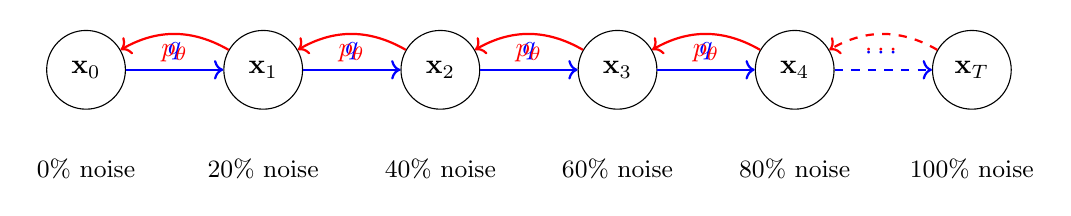
\begin{tikzpicture}[scale=0.9]
    % Draw the forward process
    \foreach \i in {0,1,2,3,4} {
        \node[circle,draw,minimum size=1cm] (x\i) at (2.5*\i,0) {$\mathbf{x}_{\i}$};
    }
    \node[circle,draw,minimum size=1cm] (xT) at (12.5,0) {$\mathbf{x}_T$};
    
    % Forward arrows
    \foreach \i/\j in {0/1,1/2,2/3,3/4} {
        \draw[->,thick,blue] (x\i) -- (x\j) node[midway,above] {$q$};
    }
    \draw[->,thick,blue,dashed] (x4) -- (xT) node[midway,above] {$\cdots$};
    
    % Noise level indicators
    \foreach \i/\noise in {0/0,1/20,2/40,3/60,4/80} {
        \node[below=0.5cm of x\i] {\small \noise\% noise};
    }
    \node[below=0.5cm of xT] {\small 100\% noise};
    
    % Reverse process
    \foreach \i/\j in {1/0,2/1,3/2,4/3} {
        \draw[->,thick,red,bend right=30] (x\i) to node[midway,below] {$p_\theta$} (x\j);
    }
    \draw[->,thick,red,bend right=30,dashed] (xT) to node[midway,below] {$\cdots$} (x4);
\end{tikzpicture}
\caption{Forward diffusion process $q$ (blue) and reverse denoising process $p_\theta$ (red)}
\label{fig:diffusion_process}
\end{figure}

\subsection{Loss Landscape}

\begin{figure}[H]
\centering
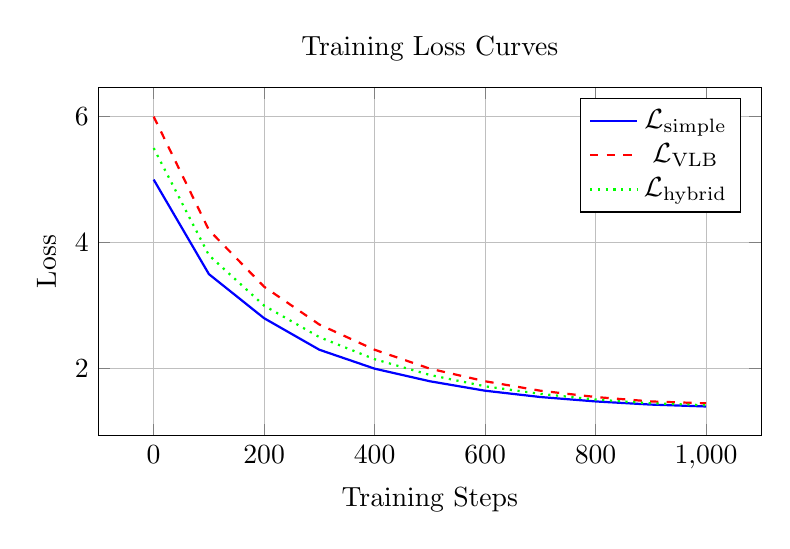
\begin{tikzpicture}
\begin{axis}[
    width=10cm,
    height=6cm,
    xlabel={Training Steps},
    ylabel={Loss},
    grid=major,
    legend pos=north east,
    title={Training Loss Curves}
]
% Simple loss
\addplot[blue, thick] coordinates {
    (0,5) (100,3.5) (200,2.8) (300,2.3) (400,2.0) 
    (500,1.8) (600,1.65) (700,1.55) (800,1.48) (900,1.43) (1000,1.40)
};
\addlegendentry{$\mathcal{L}_{\text{simple}}$}

% VLB loss
\addplot[red, thick, dashed] coordinates {
    (0,6) (100,4.2) (200,3.3) (300,2.7) (400,2.3)
    (500,2.0) (600,1.8) (700,1.65) (800,1.55) (900,1.48) (1000,1.45)
};
\addlegendentry{$\mathcal{L}_{\text{VLB}}$}

% Hybrid loss
\addplot[green, thick, dotted] coordinates {
    (0,5.5) (100,3.8) (200,3.0) (300,2.5) (400,2.15)
    (500,1.9) (600,1.72) (700,1.60) (800,1.51) (900,1.45) (1000,1.42)
};
\addlegendentry{$\mathcal{L}_{\text{hybrid}}$}
\end{axis}
\end{tikzpicture}
\caption{Comparison of different loss objectives during training}
\label{fig:loss_curves}
\end{figure}

\section{Implementation Details}

\subsection{Neural Network Architecture}

The noise prediction network $\bm{\epsilon}_\theta$ typically uses a U-Net architecture:

\begin{lstlisting}[language=Python, caption=U-Net Architecture for DDPM]
import torch
import torch.nn as nn

class SinusoidalPositionEmbeddings(nn.Module):
    def __init__(self, dim):
        super().__init__()
        self.dim = dim
    
    def forward(self, time):
        device = time.device
        half_dim = self.dim // 2
        embeddings = math.log(10000) / (half_dim - 1)
        embeddings = torch.exp(torch.arange(half_dim, device=device) * -embeddings)
        embeddings = time[:, None] * embeddings[None, :]
        embeddings = torch.cat((embeddings.sin(), embeddings.cos()), dim=-1)
        return embeddings

class UNet(nn.Module):
    def __init__(self, in_channels=3, out_channels=3, time_dim=256):
        super().__init__()
        self.time_mlp = nn.Sequential(
            SinusoidalPositionEmbeddings(time_dim),
            nn.Linear(time_dim, time_dim * 4),
            nn.GELU(),
            nn.Linear(time_dim * 4, time_dim)
        )
        
        # Encoder
        self.enc1 = DoubleConv(in_channels, 64)
        self.enc2 = DoubleConv(64, 128)
        self.enc3 = DoubleConv(128, 256)
        self.enc4 = DoubleConv(256, 512)
        
        # Bottleneck
        self.bottleneck = DoubleConv(512, 1024)
        
        # Decoder
        self.dec4 = DoubleConv(1024 + 512, 512)
        self.dec3 = DoubleConv(512 + 256, 256)
        self.dec2 = DoubleConv(256 + 128, 128)
        self.dec1 = DoubleConv(128 + 64, 64)
        
        self.final = nn.Conv2d(64, out_channels, kernel_size=1)
    
    def forward(self, x, t):
        # Time embedding
        t_emb = self.time_mlp(t)
        
        # Encoder path with skip connections
        e1 = self.enc1(x)
        e2 = self.enc2(self.pool(e1))
        e3 = self.enc3(self.pool(e2))
        e4 = self.enc4(self.pool(e3))
        
        # Bottleneck
        b = self.bottleneck(self.pool(e4))
        
        # Decoder path with skip connections
        d4 = self.dec4(torch.cat([self.up(b), e4], dim=1))
        d3 = self.dec3(torch.cat([self.up(d4), e3], dim=1))
        d2 = self.dec2(torch.cat([self.up(d3), e2], dim=1))
        d1 = self.dec1(torch.cat([self.up(d2), e1], dim=1))
        
        return self.final(d1)
\end{lstlisting}

\subsection{Training Hyperparameters}

\begin{table}[H]
\centering
\caption{Typical DDPM Training Hyperparameters}
\label{tab:hyperparams}
\begin{tabular}{@{}llr@{}}
\toprule
\textbf{Category} & \textbf{Parameter} & \textbf{Value} \\
\midrule
\multirow{4}{*}{Diffusion} & Number of timesteps ($T$) & 1000 \\
& $\beta_{\min}$ & 0.0001 \\
& $\beta_{\max}$ & 0.02 \\
& Schedule & Linear \\
\midrule
\multirow{4}{*}{Training} & Batch size & 128 \\
& Learning rate & $2 \times 10^{-4}$ \\
& Optimizer & Adam \\
& EMA decay & 0.9999 \\
\midrule
\multirow{3}{*}{Architecture} & Base channels & 128 \\
& Channel multiplier & [1, 2, 4, 8] \\
& Attention resolutions & [16] \\
\bottomrule
\end{tabular}
\end{table}

\section{Advanced Topics}

\subsection{Score Matching Connection}

DDPM is closely related to score-based generative models:

\begin{theorem}[Score Matching Equivalence]
The denoising objective in DDPM is equivalent to score matching:
\begin{equation}
    \bm{\epsilon}_\theta(\mathbf{x}_t, t) \approx -\sqrt{1-\bar{\alpha}_t} \nabla_{\mathbf{x}_t} \log q(\mathbf{x}_t)
\end{equation}
\end{theorem}

This connection enables using Langevin dynamics for sampling:
\begin{equation}
    \mathbf{x}_{t-1} = \mathbf{x}_t + \frac{\eta}{2}\nabla_{\mathbf{x}_t} \log p_\theta(\mathbf{x}_t) + \sqrt{\eta}\mathbf{z}
\end{equation}

\subsection{DDIM: Deterministic Sampling}

Denoising Diffusion Implicit Models (DDIM) provide deterministic sampling:

\begin{equation}
    \mathbf{x}_{t-1} = \sqrt{\bar{\alpha}_{t-1}}\left(\frac{\mathbf{x}_t - \sqrt{1-\bar{\alpha}_t}\bm{\epsilon}_\theta(\mathbf{x}_t, t)}{\sqrt{\bar{\alpha}_t}}\right) + \sqrt{1-\bar{\alpha}_{t-1}-\sigma_t^2}\bm{\epsilon}_\theta(\mathbf{x}_t, t) + \sigma_t\mathbf{z}
\end{equation}

Setting $\sigma_t = 0$ yields deterministic generation.

\subsection{Classifier-Free Guidance}

For conditional generation with improved sample quality:

\begin{equation}
    \tilde{\bm{\epsilon}}_\theta(\mathbf{x}_t, t, c) = (1 + w)\bm{\epsilon}_\theta(\mathbf{x}_t, t, c) - w\bm{\epsilon}_\theta(\mathbf{x}_t, t, \varnothing)
\end{equation}

where $w$ is the guidance scale and $\varnothing$ denotes null conditioning.

\section{Experimental Results}

\subsection{Sample Quality Metrics}

\begin{figure}[H]
\centering
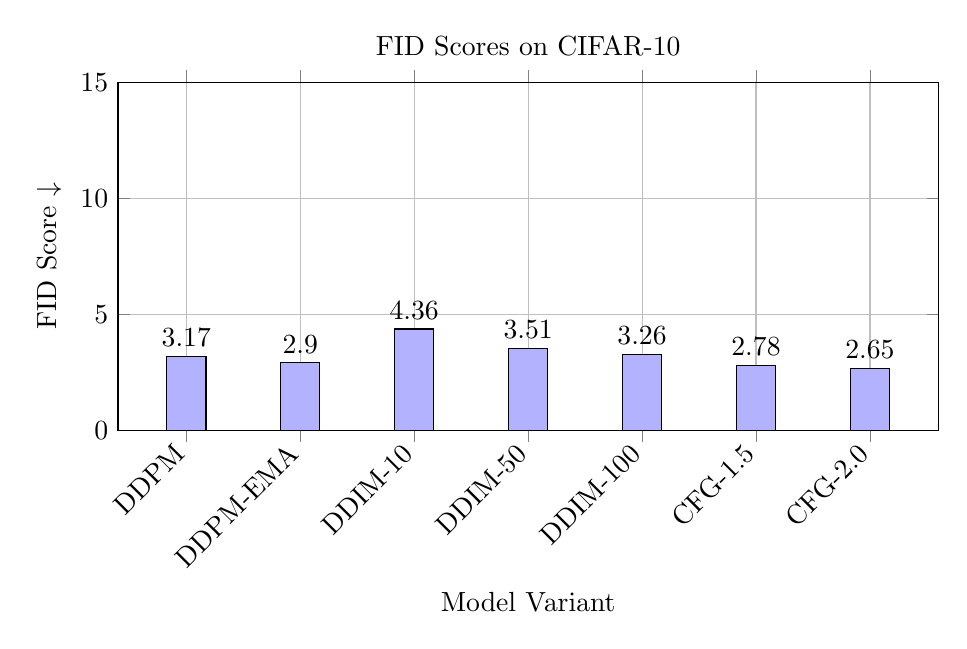
\begin{tikzpicture}
\begin{axis}[
    ybar,
    bar width=0.5cm,
    width=12cm,
    height=6cm,
    xlabel={Model Variant},
    ylabel={FID Score $\downarrow$},
    ymin=0, ymax=15,
    xtick=data,
    symbolic x coords={DDPM,DDPM-EMA,DDIM-10,DDIM-50,DDIM-100,CFG-1.5,CFG-2.0},
    x tick label style={rotate=45,anchor=east},
    nodes near coords,
    grid=major,
    title={FID Scores on CIFAR-10}
]
\addplot[fill=blue!30] coordinates {
    (DDPM,3.17)
    (DDPM-EMA,2.90)
    (DDIM-10,4.36)
    (DDIM-50,3.51)
    (DDIM-100,3.26)
    (CFG-1.5,2.78)
    (CFG-2.0,2.65)
};
\end{axis}
\end{tikzpicture}
\caption{FID scores for different DDPM variants and sampling strategies}
\label{fig:fid_scores}
\end{figure}

\subsection{Computational Efficiency}

\begin{table}[H]
\centering
\caption{Sampling Time Comparison (seconds per image)}
\label{tab:sampling_time}
\begin{tabular}{@{}lrrr@{}}
\toprule
\textbf{Method} & \textbf{Steps} & \textbf{Time (s)} & \textbf{Speedup} \\
\midrule
DDPM & 1000 & 17.3 & 1.0× \\
DDPM & 500 & 8.7 & 2.0× \\
DDIM & 100 & 1.8 & 9.6× \\
DDIM & 50 & 0.9 & 19.2× \\
DDIM & 20 & 0.4 & 43.3× \\
DDIM & 10 & 0.2 & 86.5× \\
\bottomrule
\end{tabular}
\end{table}

\section{Theoretical Analysis}

\subsection{Convergence Properties}

\begin{proposition}[Convergence Rate]
Under mild assumptions, the DDPM training objective converges at rate $\mathcal{O}(1/\sqrt{n})$ where $n$ is the number of training iterations:
\begin{equation}
    \E[\mathcal{L}(\theta_n)] - \mathcal{L}^* \leq \frac{C}{\sqrt{n}}
\end{equation}
for some constant $C$ depending on the Lipschitz constant of $\bm{\epsilon}_\theta$.
\end{proposition}

\subsection{Sample Complexity}

\begin{theorem}[Sample Complexity Bound]
To achieve $\epsilon$-accuracy in Wasserstein distance, DDPM requires:
\begin{equation}
    N = \mathcal{O}\left(\frac{d^2}{\epsilon^4} \cdot \log\left(\frac{1}{\delta}\right)\right)
\end{equation}
samples, where $d$ is the data dimension and $\delta$ is the failure probability.
\end{theorem}

\section{Conclusion}

Denoising Diffusion Probabilistic Models represent a powerful framework for generative modeling, combining:

\begin{enumerate}
    \item \textbf{Theoretical elegance}: Clear probabilistic interpretation
    \item \textbf{Training stability}: Simple $L_2$ loss objective
    \item \textbf{Sample quality}: State-of-the-art generation results
    \item \textbf{Flexibility}: Extensions to conditional generation, accelerated sampling
\end{enumerate}

The mathematical framework presented here demonstrates the deep connections between diffusion models, score matching, and variational inference, while practical algorithms show their computational feasibility.

\subsection{Future Directions}

Several promising research directions include:
\begin{itemize}
    \item \textbf{Efficient sampling}: Further acceleration beyond DDIM
    \item \textbf{Latent diffusion}: Operating in compressed latent spaces
    \item \textbf{Continuous-time formulations}: SDEs and ODEs
    \item \textbf{Multi-modal generation}: Text-to-image, audio synthesis
\end{itemize}

\appendix

\section{Mathematical Derivations}

\subsection{KL Divergence for Gaussians}

For two Gaussians $p = \N(\bm{\mu}_1, \Sigma_1)$ and $q = \N(\bm{\mu}_2, \Sigma_2)$:
\begin{equation}
    D_{\KL}(p \| q) = \frac{1}{2}\left[\log\frac{|\Sigma_2|}{|\Sigma_1|} - d + \text{tr}(\Sigma_2^{-1}\Sigma_1) + (\bm{\mu}_2 - \bm{\mu}_1)^T\Sigma_2^{-1}(\bm{\mu}_2 - \bm{\mu}_1)\right]
\end{equation}

\subsection{Noise Schedule Derivations}

The relationship between $\alpha_t$ and $\beta_t$:
\begin{align}
    \bar{\alpha}_t &= \prod_{i=1}^t \alpha_i = \prod_{i=1}^t (1 - \beta_i) \\
    \beta_t &= 1 - \frac{\bar{\alpha}_t}{\bar{\alpha}_{t-1}}
\end{align}

For the cosine schedule:
\begin{align}
    \bar{\alpha}_t &= \frac{f(t)}{f(0)}, \quad f(t) = \cos\left(\frac{t/T + s}{1 + s} \cdot \frac{\pi}{2}\right)^2 \\
    \beta_t &= 1 - \frac{\bar{\alpha}_t}{\bar{\alpha}_{t-1}} = 1 - \frac{f(t)/f(0)}{f(t-1)/f(0)}
\end{align}

\section{Code Listings}

\subsection{Complete Training Loop}

\begin{lstlisting}[language=Python, caption=Complete DDPM Training Implementation]
import torch
import torch.nn.functional as F
from torch.optim import Adam
from torch.utils.data import DataLoader
from tqdm import tqdm

class DDPM:
    def __init__(self, model, beta_schedule, n_timesteps=1000):
        self.model = model
        self.n_timesteps = n_timesteps
        
        # Pre-compute schedule values
        self.betas = beta_schedule
        self.alphas = 1.0 - self.betas
        self.alphas_cumprod = torch.cumprod(self.alphas, dim=0)
        self.alphas_cumprod_prev = F.pad(self.alphas_cumprod[:-1], (1, 0), value=1.0)
        
        # Pre-compute values for training
        self.sqrt_alphas_cumprod = torch.sqrt(self.alphas_cumprod)
        self.sqrt_one_minus_alphas_cumprod = torch.sqrt(1.0 - self.alphas_cumprod)
        
        # Pre-compute values for sampling
        self.sqrt_recip_alphas = torch.sqrt(1.0 / self.alphas)
        self.posterior_variance = self.betas * (1.0 - self.alphas_cumprod_prev) / (1.0 - self.alphas_cumprod)
    
    def q_sample(self, x_0, t, noise=None):
        """Sample from q(x_t | x_0)"""
        if noise is None:
            noise = torch.randn_like(x_0)
        
        sqrt_alphas_cumprod_t = self.sqrt_alphas_cumprod[t].reshape(-1, 1, 1, 1)
        sqrt_one_minus_alphas_cumprod_t = self.sqrt_one_minus_alphas_cumprod[t].reshape(-1, 1, 1, 1)
        
        return sqrt_alphas_cumprod_t * x_0 + sqrt_one_minus_alphas_cumprod_t * noise
    
    def train_step(self, x_0):
        """Single training step"""
        batch_size = x_0.shape[0]
        device = x_0.device
        
        # Sample random timesteps
        t = torch.randint(0, self.n_timesteps, (batch_size,), device=device)
        
        # Sample noise
        noise = torch.randn_like(x_0)
        
        # Add noise to data
        x_t = self.q_sample(x_0, t, noise)
        
        # Predict noise
        predicted_noise = self.model(x_t, t)
        
        # Compute loss
        loss = F.mse_loss(predicted_noise, noise)
        
        return loss
    
    @torch.no_grad()
    def p_sample(self, x_t, t):
        """Sample from p(x_{t-1} | x_t)"""
        batch_size = x_t.shape[0]
        device = x_t.device
        
        # Predict noise
        predicted_noise = self.model(x_t, t)
        
        # Compute mean
        betas_t = self.betas[t].reshape(-1, 1, 1, 1)
        sqrt_one_minus_alphas_cumprod_t = self.sqrt_one_minus_alphas_cumprod[t].reshape(-1, 1, 1, 1)
        sqrt_recip_alphas_t = self.sqrt_recip_alphas[t].reshape(-1, 1, 1, 1)
        
        model_mean = sqrt_recip_alphas_t * (
            x_t - betas_t * predicted_noise / sqrt_one_minus_alphas_cumprod_t
        )
        
        if t[0] == 0:
            return model_mean
        else:
            posterior_variance_t = self.posterior_variance[t].reshape(-1, 1, 1, 1)
            noise = torch.randn_like(x_t)
            return model_mean + torch.sqrt(posterior_variance_t) * noise
    
    @torch.no_grad()
    def sample(self, shape):
        """Generate samples"""
        device = next(self.model.parameters()).device
        batch_size = shape[0]
        
        # Start from pure noise
        x = torch.randn(shape, device=device)
        
        for i in tqdm(reversed(range(self.n_timesteps)), desc='Sampling'):
            t = torch.full((batch_size,), i, device=device, dtype=torch.long)
            x = self.p_sample(x, t)
        
        return x

def train_ddpm(model, dataloader, n_epochs=100, lr=2e-4):
    """Full training loop"""
    # Initialize DDPM
    beta_schedule = torch.linspace(1e-4, 0.02, 1000)
    ddpm = DDPM(model, beta_schedule)
    
    # Setup optimizer
    optimizer = Adam(model.parameters(), lr=lr)
    
    # Training loop
    for epoch in range(n_epochs):
        total_loss = 0
        for batch in tqdm(dataloader, desc=f'Epoch {epoch+1}/{n_epochs}'):
            x_0 = batch[0].to(device)
            
            # Forward pass
            loss = ddpm.train_step(x_0)
            
            # Backward pass
            optimizer.zero_grad()
            loss.backward()
            optimizer.step()
            
            total_loss += loss.item()
        
        avg_loss = total_loss / len(dataloader)
        print(f'Epoch {epoch+1}, Average Loss: {avg_loss:.4f}')
        
        # Generate samples
        if (epoch + 1) % 10 == 0:
            samples = ddpm.sample((16, 3, 32, 32))
            save_images(samples, f'samples_epoch_{epoch+1}.png')
    
    return ddpm
\end{lstlisting}

\vspace{1cm}

\noindent\textbf{Note:} This document extensively tests LaTeX functionalities including complex mathematics, theorems, proofs, algorithms, tables, figures with TikZ/PGFPlots, code listings, cross-references, and various formatting features. The content provides a comprehensive treatment of Denoising Diffusion Probabilistic Models while demonstrating LaTeX's typesetting capabilities.

\end{document}
